\section{\mc 目的}
\subsection{\mc モチベーション}
特徴量抽出手法や分類器を拡張する方針とは異なり、
より綿密にEEGの解析を行うことで性能の向上を達成しようとする試みも続いている\cite{脳波解析BCI,脳波分析BCI,ERSBCI}。
EEGではBCIに限らず、頭皮領域と周波数帯域に関しての研究が盛んに行われてきたため、
特徴量抽出を行う場合にも電極と周波数に着目する場合が多い。
特にERDは特定の周波数における電位の減少であるため、
スペクトル解析と時間周波数解析が有効利用でき、
現在も運動想起型BCIのための研究が行われている\cite{時間周波数解析の比較}。

一方で現在、運動想起型BCIで高い性能を誇る手法は
統計的信号処理や機械学習手法に基づいている。
このことは不可解なことではない。
綿密なEEGの解析を実施するか否かに関わらず、
左手を動作させる場合と右手を動作させる場合とでは脳の活動は事実異なっているためである。
タスク間でのEEGの違いを可視化したい場合や、
脳機能自体を解明したい場合には綿密なEEGの解析は有効であるが
、その際には解析はあくまで人間が解釈する手段であり、
解析のために処理された信号がそのまま特徴量として有望だとは限らない。
% 本論文では、BCIが動作するための特徴量抽出を
% 人間が解釈できる形で与える必要はないと主張する。
なぜなら人間がデータを解釈、あるいは可視化できるような形に加工することで
分類に有用な情報が失われている可能性もあるためである。

しかし、運動想起型BCIを構築するための特徴量抽出手法、
分類手法は数多く存在する。代表的なものを以下に記す。
この中の幾つかは第\ref{chapter:BCIのための要素技術}章にて解説する。
\begin{itemize}
    \item Laplacian Filter(LF)
    \item Principal Component Analysis(PCA)
    \item Independent Component Analysis(ICA)
    \item Canonical Correspondence Analysis(CCA)
    \item Common Spartial Pattern(CSP)
    \item バンドパスフィルタバンク
    \item フーリエ変換
    \item ウェーブレット変換
    \item 自己回帰モデル
    \item Emperical Mode Decomposition(EMD)
    \item Linear Discriminat Analysis(LDA)
    \item Support Vector Machine(SVM)
    \item Logistic Regression(LR)
\end{itemize}
これらの手法はBCIの構成要素として組み込まれるが
数多くある手法の中から個々人に応じて、
あるいはタスクに応じて適切に組み合わせるのは容易ではない。
その中、FBCSPはバンドパスフィルタバンクとCSP
及びLDAを組み合わせた数少ない成功例であり、
現在でもバンドパスフィルタとCSPを基本とした
派生手法が提案され続けている\cite{sparsemethod,bootCSP}。
しかし、数多くの手法が提案されている中で、
FBCSP以降は運動想起型BCIとしての決定的なアーキテクチャは提案されていないと言える。

\subsection{\mc 達成目標}
本研究では音声認識や画像認識の分野で高い性能を発揮している
ニューラルネットワークに着目する。
ニューラルネットワークは学習時の計算量が膨大であることから、
長い間研究が滞っていたが、近年の計算機の発展により応用研究に用いられるようになり、
人間の設計した分類器を凌駕する性能の高さから注目が集まっている。

ニューラルネットワークの実体は巨大な合成関数であり、
事実上単なるパラメトリックな数理モデルである。
しかし、誤差逆伝播学習によって原理上極めて
深い合成関数の形式であっても学習が可能であるため、
問題に応じてネットワーク構造の設計を適切に行うことで、
特徴量抽出と分類を同時に達成できる可能性がある。
更にその学習のアルゴリズム自体は極めて単純であるが効果的に働き\cite{CheapLearning}、
再学習可能であるため有用なニューラルネットワークの構造が発見された場合にその再利用性が高い。
加えて、ニューラルネットワークの深層構造によって高い性能が引き出されること\cite{DeepvsShallow}や、
モデルの複雑さと比較して最適化問題の目的関数は病理的ではない、
あるいは病理的な形状を回避できることが示唆されるようになった\cite{ディープローカルミニマム}。

従って、運動想起型BCIに適したニューラルネットワークの検討を行い、
基礎的な構造を確立することは有益であると考え、本研究の目的とする。

\subsection{\mc 技術的貢献}
典型的な運動想起型BCIは、運動想起に関連しているEEGを取り出すための前処理\(\cal H(\cdot)\)
によってEEGの生データ\(X\)から\(\hat X\)を獲得することが一般的である。
\begin{equation}
    \hat X = {\cal H}(X)
    \label{eq:bandpass}
\end{equation}
次に、運動想起に関連している空間的な情報を抽出する処理を\(f(\cdot)\)を適用し、
特徴量\(Z\)を取り出す。
\begin{equation}
    Z = f(\hat X)
    \label{eq:spatfilter}
\end{equation}
続いて\(Z\)に対して、
運動想起部位\(Y\)を出力する分類器\(g(\cdot)\)を準備することで、運動想起BCIが構成されている。
\begin{equation}
    Y = g(Z)
    \label{eq:classifier}
\end{equation}
従って、BCIはEEG\(X\)を引数とした合成関数という形式を取る。
\begin{equation}
    Y = (g\circ f \circ {\cal H})(X)
    \label{eq:bci_gosei}
\end{equation}
実際に合成関数としてどのようなものが選択されるか、
EEGがどのように測定されるかはタスクに依存するが、
典型的なCSPを用いたBCIでは\(X\)を運動想起時のEEG、\(\cal H\)をバンドパスフィルタ、
\(f\)をCSP、\(g\)をLDAやSVMとして各々個別に設計する。

一方で時間周波数解析に基づくBCIでも特徴抽出として
何らかの時間周波数解析\(h(\cdot)\)が関数内に挿入され、
\begin{equation}
    Y = (g\circ h \circ f \circ {\cal H})(X)
    \label{eq:bci_gosei2}
\end{equation}
という形式で表せる。この時、\(\cal H\)や\(f\)はERDを検出するための
神経科学的な知見に基づいた設計がなされる場合もあれば、
機械学習の手法が用いられる場合もある。
更に時間周波数解析によって得られるパワースペクトログラムに対して
非負値行列分解などを用いて特徴量を抽出する試みもある\cite{kNMF,kNMF2}。
この場合も行列分解による変換を\(a(\cdot)\)と置けば
\begin{equation}
    Y = (g\circ a\circ h\circ f\circ {\cal H})(X)
    \label{eq:bci_gosei3}
\end{equation}
と表され、形式上は合成関数である。
それぞれの関数の役割を明示しなければ、BCIは単に以下の合成関数である。
\begin{equation}
    Y = (f_K\circ \cdots \circ f_1)(X)
    \label{eq:bci_gosei4}
\end{equation}
すなわちBCIは設計を終えた時には何らかの合成関数として構築されている。
実際に設計を行う際には各々の合成関数に対して関数族を仮定し、
学習やヒューリスティクスによって関数を決定し、最後に合成する。
しかしこのとき、BCIのデータの流れから明らかに関数\(f_i\)を設計するためには
\(f_{i-1}\)の設計が終了していなければならない。

一方でニューラルネットワークは万能な関数近似器である。
ニューラルネットワークの構造を与えることで適切な関数族を仮定することができれば、
誤差逆伝播学習によってEnd to EndでのBCI設計が可能となる。
BCIとして考えうる構成と、ニューラルネットワークを用いたBCIの構成図を図\ref{fig:BCIpattern}に示す。
\begin{figure}
    \centering
    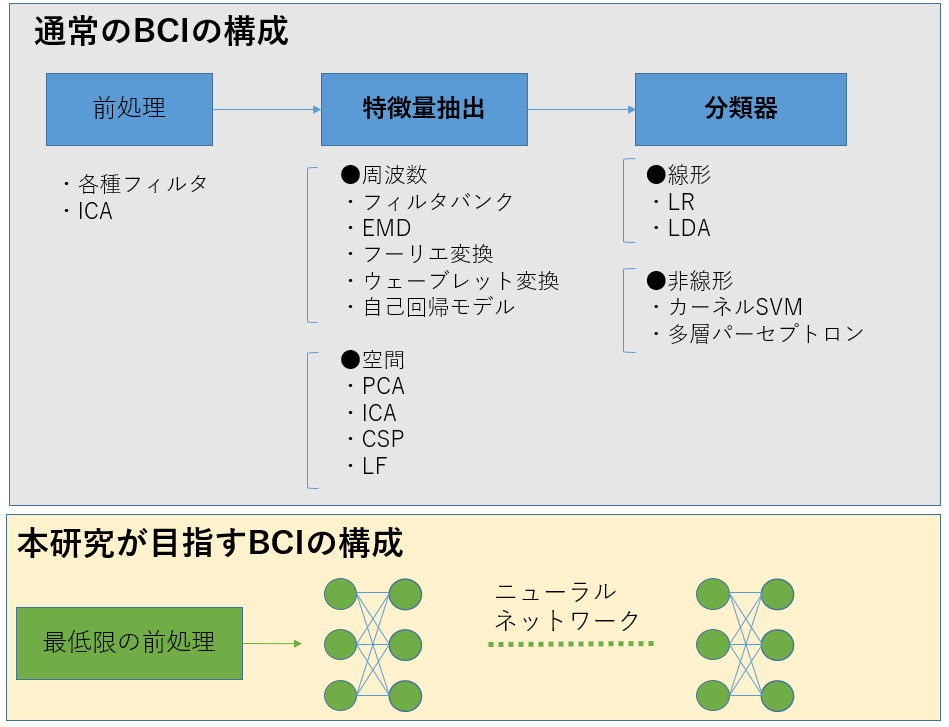
\includegraphics[width=15cm]{images/BCIpattern.PNG}
    \caption{従来のBCIの構成と本研究が目指すBCIの構成}
    \label{fig:BCIpattern}
\end{figure}

また、ニューラルネットワークの応用研究が盛んな画像認識の分野では、
既に模範的なニューラルネットワークの構造が発見されており、
大量の画像によって事前学習を行い、
達成したい認識対象を絞り込んだ後に転移学習することで
手軽に高い性能の分類器が得られる。
従って、BCIにおいて模範的なニューラルネットワークの構築により
以下の事項が達成できる可能性が示唆される。
従って研究の成果によって以下の項目において貢献することができる。
\begin{itemize}
    % \item タスク毎のEEGの解析の必要性を排除
    \item 各個人におけるEEGの解析の必要性を排除
    \item 人類に共通した一般的なBCIの基本モデル構築
\end{itemize}
また、マルチモーダルなBCIの一部としても応用可能である。

% 更に、モデルの構築も含めハイパーパラメータの存在によって
% 試行錯誤の必要性も非常に高い。
% しかし、特徴量抽出手法や分類器自体を変更しながら様々な組み合わせを検討することに比べ、
% ニューラルネットワークの調整は単純作業である。
% また今後ハイパーパラメータの調整自体を自動化する、
% あるいは学習に組み込む方法も出現する可能性がある。


